% ------------------------------------------------------------------------------
% TYPO3 Version 9.1 - What's New - Chapter "Backend User Interface" (Dutch Version)
%
% @author	Michael Schams <schams.net>
% @license	Creative Commons BY-NC-SA 3.0
% @link		http://typo3.org/download/release-notes/whats-new/
% @language	English
% ------------------------------------------------------------------------------
% LTXE-CHAPTER-UID:		07b25346-95b1df21-a6ebe09a-49f53f41
% LTXE-CHAPTER-NAME:	Backend User Interface
% ------------------------------------------------------------------------------

\section{Gebruikersinterface backend}
\begin{frame}[fragile]
	\frametitle{Gebruikersinterface backend}

	\begin{center}\huge{Hoofdstuk 1:}\end{center}
	\begin{center}\huge{\color{typo3darkgrey}\textbf{Gebruikersinterface backend}}\end{center}

\end{frame}

% ------------------------------------------------------------------------------
% LTXE-SLIDE-START
% LTXE-SLIDE-UID:		e00a440f-29873f84-81d02239-075d4fb6
% LTXE-SLIDE-ORIGIN:	e0ad33fe-9f5b1a93-218b12e9-6410e8f5 English
% LTXE-SLIDE-TITLE:		Added New Main Module Site Management
% LTXE-SLIDE-REFERENCE:	Feature-83637-AddedNewMainModuleSiteManagement.rst
% ------------------------------------------------------------------------------

\begin{frame}[fragile]
	\frametitle{Gebruikersinterface backend}
	\framesubtitle{Site beheer}

	Een nieuwe module \textbf{Site beheer} in geïntroduceerd in de TYPO3 core.
	Het hoofddoel is om functies onder te brengen die gerelateerd zijn aan de configuratie van de site,
	zoals bijvoorbeeld talen, domeinen en routering.

	\begin{columns}[T]
		\begin{column}{.4\textwidth}
			\begin{figure}\vspace*{-0.4cm}
				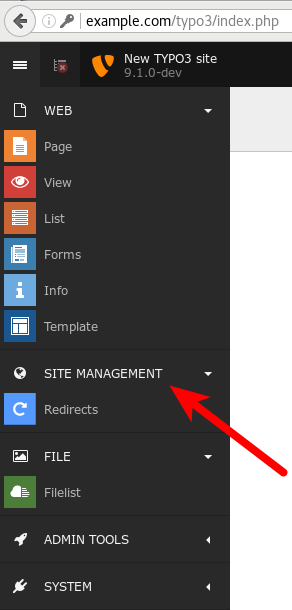
\includegraphics[width=0.45\linewidth]{BackendUserInterface/AddedNewMainModuleSiteManagement.png}
			\end{figure}
		\end{column}
		\begin{column}{.5\textwidth}
			De nieuwe systeemextensie \texttt{EXT:redirects} is het eerste onderdeel
			van deze hoofdmodule (zie volgende pagina's voor meer informatie).
		\end{column}
		\begin{column}{.1\textwidth}
		\end{column}
	\end{columns}

\end{frame}

% ------------------------------------------------------------------------------
% LTXE-SLIDE-START
% LTXE-SLIDE-UID:		85926cc1-8e1f9db9-c1657233-b9c2c080
% LTXE-SLIDE-ORIGIN:	8bd6b85d-ed8c77e3-94a40b39-e15bb504 English
% LTXE-SLIDE-TITLE:		System Extension "Redirects" Has Been Added
% LTXE-SLIDE-REFERENCE:	Feature-83631-SystemExtensionRedirectsHasBeenAdded.rst
% ------------------------------------------------------------------------------

\begin{frame}[fragile]
	\frametitle{Gebruikersinterface backend}
	\framesubtitle{Redirects}

	Deze nieuwe module stelt integrators en redacteuren in staat om redirects te configureren.
	Deze functie bevat een simpele teller (moet ingeschakeld worden) en
	redirects kunnen voor een onbeperkte of een specifieke tijd ingesteld worden.

	\begin{figure}
		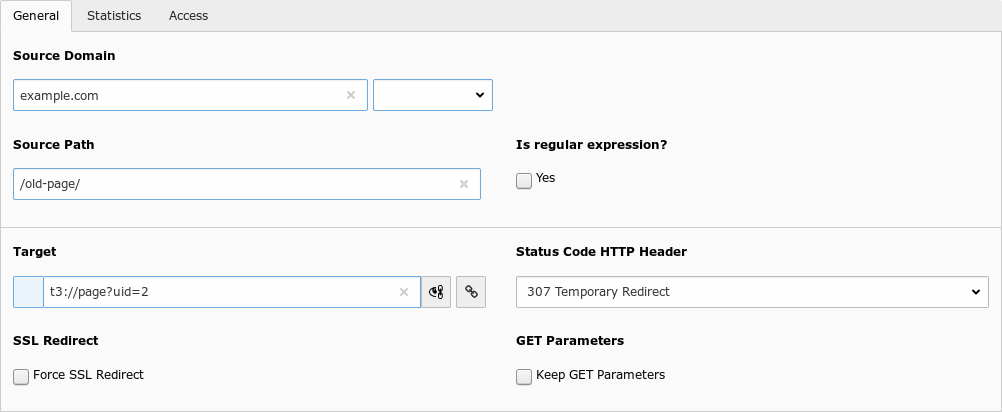
\includegraphics[width=0.8\linewidth]{BackendUserInterface/SystemExtensionRedirectsHasBeenAdded.png}
	\end{figure}

\end{frame}

% ------------------------------------------------------------------------------
% LTXE-SLIDE-START
% LTXE-SLIDE-UID:		06fda975-6ceb8992-b588dfaf-a995e9c8
% LTXE-SLIDE-ORIGIN:	e10a0f89-e91ecdb3-928841b6-1a84fc50 English
% LTXE-SLIDE-TITLE:		Show Fieldname Next To Title In Debug Mode
% LTXE-SLIDE-REFERENCE:	Feature-83461-ShowFieldnameNextToTitleInDebugMode.rst
% ------------------------------------------------------------------------------

\begin{frame}[fragile]
	\frametitle{Gebruikersinterface backend}
	\framesubtitle{Veldnamen in debug modus}

	\begin{itemize}

		\item TYPO3 integrators en ontwikkelaars hebben regelmatig te maken met invoervelden in de backend,
			bijvoorbeeld bij het instellen van de rechten of bij de configuratie van TsConfig.

		\item In plaats van in de broncode van de browser te bekijken, worden nu de veldnamen bij ieder veld
		    gegenereerd door de FormEngine.

		\item Dit geldt alleen voor gebruikers met admin rechten en de debug modus moet inschakeld zijn in TYPO3:

			\smaller
				\texttt{\$GLOBALS['TYPO3\_CONF\_VARS']['BE']['debug']}
			\normalsize

	\end{itemize}

	\begin{figure}
		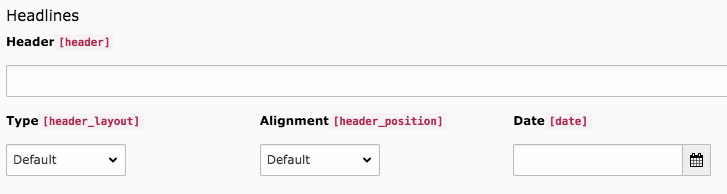
\includegraphics[width=0.60\linewidth]{BackendUserInterface/ShowFieldnameNextToTitleInDebugMode.png}
	\end{figure}

\end{frame}

% ------------------------------------------------------------------------------
